\documentclass[a4paper,11pt]{article}

%Package utilisé
\usepackage[latin1]{inputenc}
\usepackage[T1]{fontenc}
\usepackage[francais]{babel}
\usepackage[top=3cm, bottom=3cm, left=3cm, right=3cm]{geometry}
\usepackage{graphicx}
\usepackage{caption}
\usepackage{listings}
\usepackage{verbatim}
\usepackage{xcolor}
\usepackage{gensymb}
\usepackage{float}

\begin{document}


%Page de garde
\begin{titlepage}
    \vspace{-20px}
    \begin{tabular}{l}
	\textsc{Bannier} K\'evin\\
    \textsc{Loiseau} Anne-Claire
    \end{tabular}
    \hfill \vspace{10px}
\includegraphics[scale=0.1]{./images/esir.png}\\
    \vfill
    \begin{center}
        \Huge{\'Ecole sup\'erieure d'ing\'enieurs de Rennes}\\
        \vspace{1cm}
        \LARGE{3\`eme Ann\'ee}\\
        \large{Parcours IN}\\
        \vspace{0.5cm}\hrule\vspace{0.5cm}
        \LARGE{\textbf{Compte-rendu du TP n\degree 6 d'Imagerie M\'edicale}}\\
        \Large{Robotique m\'edicale : Asservissement visuel d'ultrason}
        \vspace{0.5cm}\hrule
        \vfill
        \vfill
    \end{center}
    \begin{flushleft}
        \Large{Sous l'encadrement de~:}\\
        \vspace{0.2cm}
        \large{{Alexandre} Krupa}
    \end{flushleft}
    \hfill \vspace{10px} Le 06 D\'ecembre 2016
    \vfill
\end{titlepage}



\section{Objectif du TP}

L'objectif de ce TP est de simuler le positionnement automatique d'une sonde \'echographique 2D par un robot. Cela est possible en r\'ealisant un asservisemment visuel des informations denses observ\'ees dans l'image rendue par la sonde ultrasonore, et en analysant les mouvements du patient (tel que la respiration) dans le but de les compenser automatiquement.
Pour r\'ealiser cela nous allons utiliser un simulateur de sonde ultrasonore poss\'edant 6 degr\'es de libert\'e, d\'evelopp\'e par l'\'equipe Lagadic de l'INRIA. Pour arriver \`a r\'ealiser un positionnement automatique, nous allons suivre plusieurs \'etapes divis\'ees en 13 questions, et qui suivent le d\'eroulement du cours. Nous allons donc, dans ce rapport, d\'etailler ce que nous avons r\'ealis\'e \`a chacune de ces questions.


\section{Travail r\'ealis\'e}
Avant de d\'emarrer la r\'edaction du code et les r\'eponses aux questions, nous avons lanc\'es l'outil de simulation r\'ealis\'e par l'\'equipe de l'INRIA. Cet outil ouvre plusieus fen\^etres qui sont les suivantes :
\begin{itemize}
\item L'image actualis\'e de l'ultrason. Cette image doit prendre en compte les battements simul\'es du coeur, et doit donc les compenser pour garder la zone d'int\'er\^et dans le champ de vision.
\item L'image d\'esir\'e. Cette image n'est pas cens\'e bouger par la suite, elle montre la zone d'int\'er\^et s\'el\'ectionn\'e.
\item L'image diff\'erence entre les deux pr\'ec\'edentes.
\item Courbe de vitesse de d\'eplacement de la sonde (en translation et en rotation)
\item Courbe d'erreur de position de la sonde (en translation et en rotation)
\item Courbe d'erreur de la fonction de co\^ut. Cela repr\'esente l'erreur de la compensation par rapport au mouvement r\'eellement effectu\'e.
\end{itemize}

\subsection{Question 1}
Dans cette partie, nous allons appliquer les 6 degr\'es de libert\'e de la sonde, dans le but de simuler les mouvements du patient. Voici le code qui nous permet de r\'ealiser cela :
\begin{verbatim}
double ampliture_t = 0.020;
double ampliture_r = 20.0;

object_velocity[0] = ampliture_t*sin(2*M_PI*(1.0/5.0)*time);
object_velocity[1] = ampliture_t*sin(2*M_PI*(1.0/5.0)*time);
object_velocity[2] = ampliture_t*sin(2*M_PI*(1.0/5.0)*time);

object_velocity[3] = vpMath::rad(ampliture_r) * sin( 2*M_PI*(1.0/5.0)*time);
object_velocity[4] = vpMath::rad(ampliture_r) * sin( 2*M_PI*(1.0/5.0)*time);
object_velocity[5] = vpMath::rad(ampliture_r) * sin( 2*M_PI*(1.0/5.0)*time);
\end{verbatim}

Object\_velocity repr\'esente le mouvement de la sonde, et donc ses 6 degr\'es de libert\'e. Nous avons appliqu\'e ici une p\'eriode sinuso\"idale de 5 secondes pour une amplitude de 0.005 m\`etre/secondes, que l'on a transform\'e en rad/sec.\\

Le r\'esultat que nous obtenons s'applique directement sur l'image actualis\'e de l'ultrason, ce qui modifie \'egalement l'image de diff\'erence, et la courbe d'erreur de pose de la sonde. Voici ce que nous observons :
\begin{figure}[!h]
	\centering
		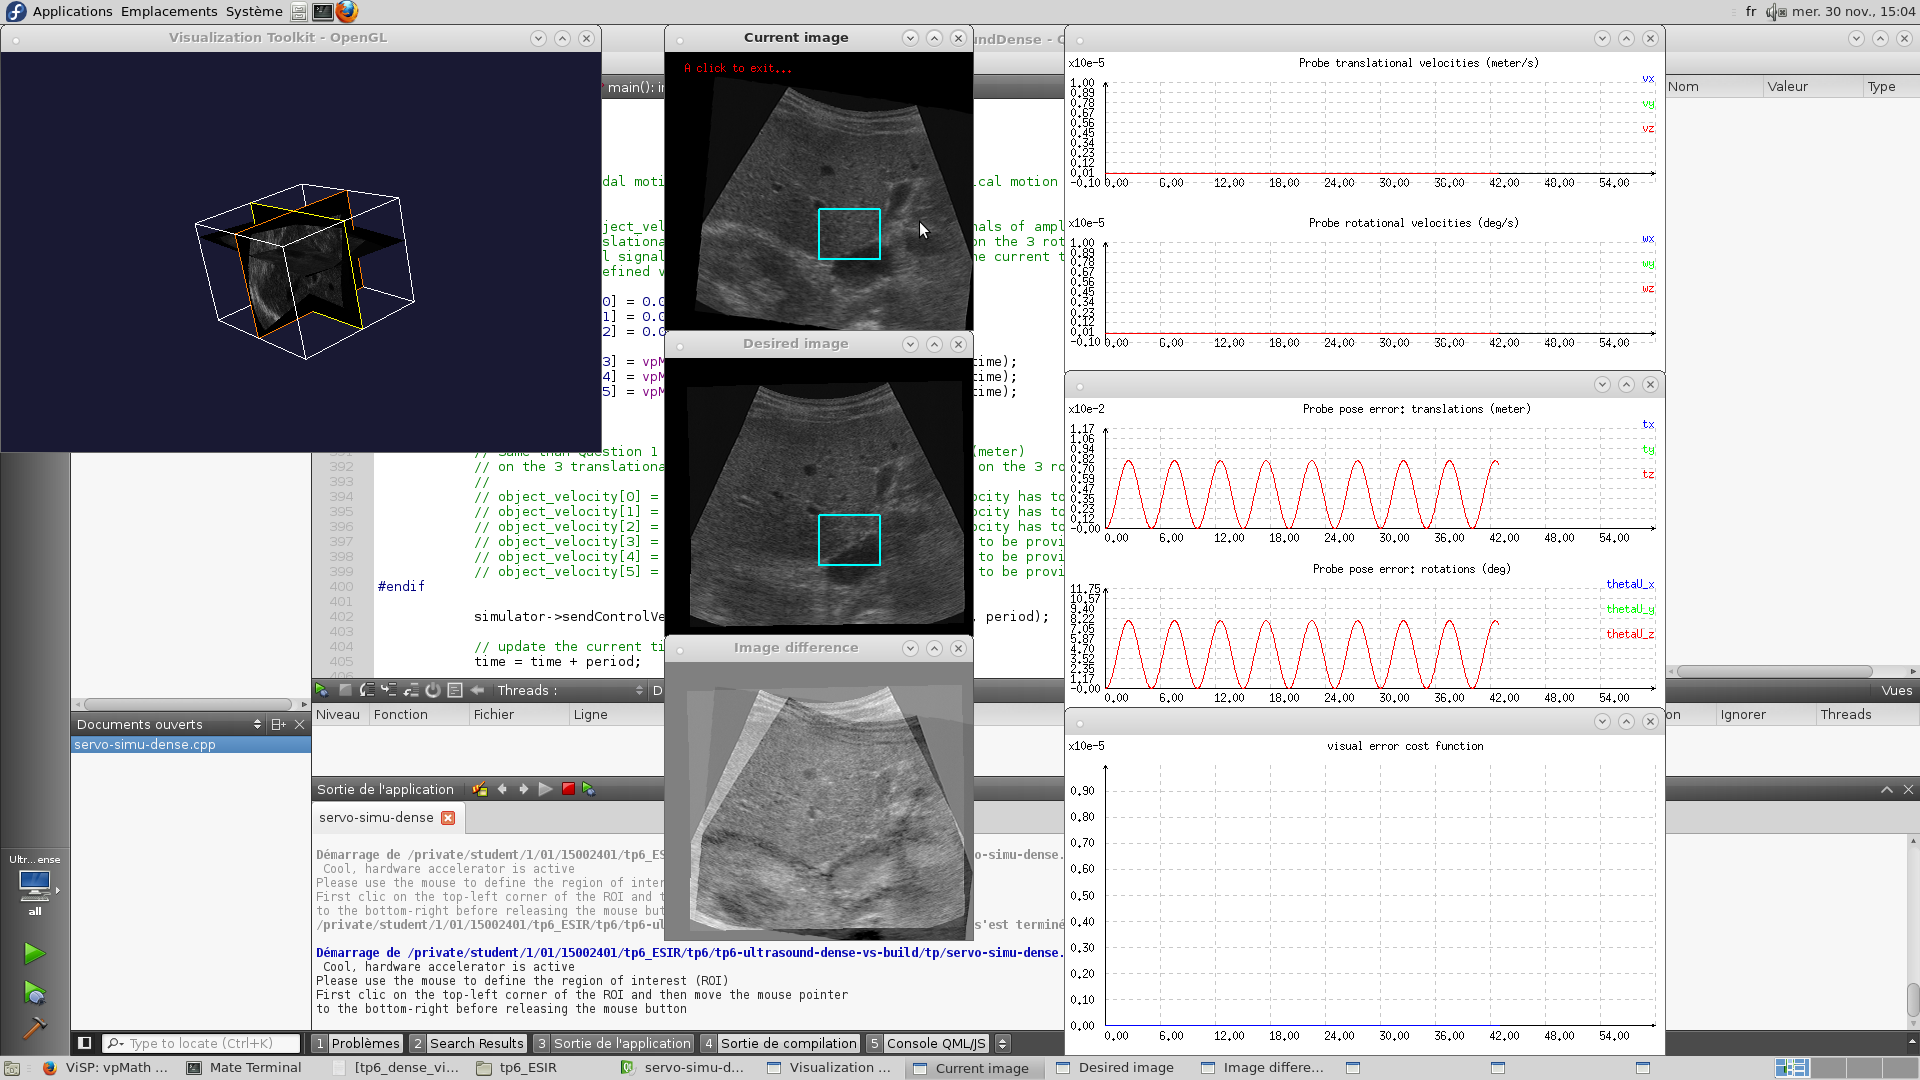
\includegraphics[width=1.0\textwidth]{./images/question1.png}
	\caption{Observation des mouvements simul\'es du patient}
	\label{mvtPatient}
\end{figure}

La Figure \ref{mvtPatient} montre l'\'etat du patient \`a un instant t. En effet, les mouvements sont continus, ce que nous montre bien la courbe. Nous observons sur cette Figure \ref{mvtPatient} une diff\'erence assez \'elev\'e entre l'image actuelle du mouvement du patient, et l'image d\'esir\'ee, c'est \`a dire l'image initiale. Cela est normal, car aucune compensation automatique n'est r\'ealis\'e pour le moment, il y a seulement le battement de c\oe ur qui est simul\'e. Ce battement de c\oe ur simul\'e par ailleurs n'est pas vraiment r\'ealiste car sa mani\'ere de bouger est r\'ealis\'e par des sinus, ce qui donne un r\'esultat tr\`es peu naturel. Nous obtenons ainsi une erreur identique entre la rotation et la translation, et cela est normal puisque rien n'est compens\'e ou m\^eme appris.
Dans cette simulation, la zone d'int\'er\^et a peu d'importance puisque nous l'avons dit, aucun mouvement n'est actuellement compens\'e en fonction de cette zone, seulement la simualtion des battements du c\oe ur est effectu\'e.


\subsection{Question 2}
Nous souhaitons d\'esormais r\'ecup\'erer et sauvegarder le contenu de la zone d'int\'er\^et initiale. Pour cela, nous allons r\'ecup\'erer le contenu de la zone dans l'image d\'esir\'ee, et donc copier l'intensit\'e des pixels de la zone concern\'ee. Ainsi, malgr\'e les mouvements du c\oe ur, la zone d'int\'er\^et est sauvegard\'e d\'es l'initialisation et va ainsi pouvoir \^etre compar\'e \`a la zone correspondante dans l'image actualis\'e de la sonde.\\

Voici notre code permettant cela :
\begin{verbatim}
for(int i=0; i<ROI_height; i++) 
{
    for(int j=0; j<ROI_width; j++) 
    {
        DesiredFeatures[i*ROI_width+j] = simulator->Image(i+Hmin, j+Wmin);
    }
}
\end{verbatim}
Pour chaque pixel appartenant \`a cette zone d'int\'er\^et, nous r\'ecup\'erons son intensit\'e.

\subsection{Question 3}
Nous souhaitons d\'esormais calculer la matrice d'int\'eraction, et pour cela calculer le gradient 3d de l'image. Pour le calculer, nous devons appliquer 9 patchs au total, 3 par coordonn\'ees (x, y ou z), puis un patch par image : l'image courant, l'image pr\'ec\'edente et l'image suivante. \\

Voici notre code permettant cela :
\begin{verbatim}
vpMatrix patchX(3,3);
patchX[0][0] = -1;  patchX[1][0] = -2;  patchX[2][0] = -1;
patchX[0][1] = 0;   patchX[1][1] = 0;   patchX[2][1] = 0;
patchX[0][2] = 1;   patchX[1][2] = 2;   patchX[2][2] = 1;

vpMatrix patchY = patchX.transpose();

vpMatrix patchZ(3,3);
patchZ[0][0] = 1;  patchZ[1][0] = 2;  patchZ[2][0] = 1;
patchZ[0][1] = 2;   patchZ[1][1] = 4;   patchZ[2][1] = 2;
patchZ[0][2] = 1;   patchZ[1][2] = 2;   patchZ[2][2] = 1;

for(int i=Hmin; i<Hmax; i++) 
{
    for(int j=Wmin; j<Wmax; j++) 
    {
        double img0Fx = ApplyPatch(2*patchX, img0, i, j);
        double img0Fy = ApplyPatch(2*patchY, img0, i, j);
        double img0Fz = 0;

        double imgaFx = ApplyPatch(patchX, imga, i, j);
        double imgaFy = ApplyPatch(patchY, imga, i, j);
        double imgaFz = ApplyPatch(-patchZ, imga, i, j);
	
        double imgbFx = ApplyPatch(patchX, imgb, i, j);
        double imgbFy = ApplyPatch(patchY, imgb, i, j);
        double imgbFz = ApplyPatch(patchZ, imgb, i, j);

        dIdx[i][j] = img0Fx + imgaFx +  imgbFx;
        dIdy[i][j] = img0Fy + imgaFy +  imgbFy;
        dIdz[i][j] = img0Fz + imgaFz +  imgbFz;
    }
}
\end{verbatim}

La premi\`ere chose \`a noter est que nous calculons ce gradient 3D uniquement sur la zone d'int\'er\^et car cela nous permet de gagner en temps de calcul sachant que ce calcul ne sera utile par la suite que dans cette zone l\`a. C'est donc \'eviter du temps de calcul inutile. \\
Le second point \`a voir sur ce code est que pour appliquer le patch sur une image, nous avons pr\'ef\'er\'e cr\'eer une m\'ethode \`a part. Cela nous permet d'avoir une meilleure visibilit\'e sur notre code concernant cette fonction de calcul du gradient 3D de l'image. En effet, comme il y a 9 patchs \`a appliquer, ce qui correspond \`a 9 fois le m\^eme traitement sur des donn\'ees diff\'erentes, il nous a paru logique de r\'ealiser ce traitement dans une nouvelle fonction. Cette fonction est la suivante :

\begin{verbatim}
/**
 * @brief usImageGradient::ApplyPatch This method apply a patch to a point 
 * (i, j) in a image img
 * @param patch : the patch to apply (ex : a 3x3 image)
 * @param img : the original image
 * @param i : coordonate i of the point
 * @param j : coordonate j of the point
 * @return the result of the patch applying to this point
 */
double usImageGradient::ApplyPatch(const vpMatrix &patch, 
vpImage<unsigned char> &img, int & i, int & j) 
{
    double result = 0;

    for(int iPatch = -(int)(patch.getRows()/2); iPatch <= (int)patch.getRows()/2; 
        iPatch++) 
    {
        for(int jPatch = -(int)(patch.getCols()/2); jPatch <= (int)patch.getCols()/2; 
            jPatch++) 
        {
            result += patch[iPatch+patch.getRows()/2][jPatch+patch.getCols()/2] 
            		  * img[i+iPatch][j+jPatch];
        }
    }
    return result;
}
\end{verbatim}
Cette fonction effectue un parcours du patch (une matrice 3x3), et calcule la nouvelle valeur au point (i,j) de l'image. Maintenant que notre gradient 3D est calcul\'e, nous allons pouvoir impl\'ementer la matrice d'int\'eraction.

\subsection{Question 4}
La matrice d'int\'eraction repr\'esente les variations d'intensit\'e des pixels par rapport au d\'eplacement de la sonde. C'est \`a dire comment \'evolue l'image, et donc l'intensit\'e de ses pixels, en fonction du mouvement de la sonde. C'est donc cette matrice qui va \^etre \`a la base de la compensation de mouvement? \\

Voici notre code calculant cette matrice d'int\'eraction :
\begin{verbatim}
int k=0;
for(int i=0;i<ROIH; i++) 
{
    for(int j=0; j<ROIW; j++) 
    {
        Ls[k][0] = dIdx[Hmin + i ][ Wmin + j];
        Ls[k][1] = dIdy[Hmin + i ][ Wmin + j];
        Ls[k][2] = dIdz[Hmin + i ][ Wmin + j];

        double x = sx*((Wmin + j)-(imgW/2));
        double y = sy*((Hmin + i)-(imgH/2));

        Ls[k][3] = y*Ls[k][2];
        Ls[k][4] = -x*Ls[k][2];
        Ls[k][5] = x*Ls[k][1] - y*Ls[k][0];
        k++;
    }
}
\end{verbatim}
Le code ci-dessus est la mise en application des formules math\'ematiques vues en cours, et rappel\'ees dans le sujet de TP. Comme pour le gradient 3D, nous calculons la matrice d'int\'eraction uniquement sur la zone d'int\'er\^et, car c'est le seul endroit o\`u nous allons v\'erifier la r\'eaction de la sonde par rapport aux battements de c\oe ur. Le calcul sur toute l'image n'aurait donc pas d'int\'er\^et et ferait perdre du temps de calcul, or la sonde doit \^etre capable de se d\'eplacer en temps r\'eel. 

\subsection{Question 5}
Nous souhaitons d\'esormais r\'ecup\'erer le contenu de la zone d'int\'er\^et en fonction du mouvement de la sonde. Comme pour la question 2, nous allons sauvegarder l'intensit\'e des pixels de cette zone. Cela nous permettra donc de pouvoir les comparer et rectifier le mouvement de la sonde. Voici donc le code nous permettant cela :
\begin{verbatim}
for(int i=0; i<ROI_height; i++) 
{
    for(int j=0; j<ROI_width; j++) 
    {
        CurrentFeatures[i*ROI_width+j] = simulator->Image(i+Hmin, j+Wmin);
    }
}
\end{verbatim}
Il s'agit du m\^eme code que pour la question 2, \`a ceci pr\`es que nous n'enregistrons pas l'information dans la m\^eme variable, et que ce code est r\'ealis\'e \`a chaque actualisation de l'image. Mais concr\`etement le but recherch\'e reste identique, c'est pourquoi nous avons r\'eutilis\'e ce code.

\subsection{Question 6}
Nous souhaitons d\'esormais bouger la sonde de sorte \`a compenser les battements du c\oe ur. Pour cela nous allons utiliser la matrice d'int\'eraction que nous venons de calculer, car elle nous donne des informations tr\`es int\'eressantes sur la variation des pixels en fonction des battements du c\oe ur. Nous calculons ce mouvment \`a effectuer gr\^ace \`a une formule math\'ematiques du cours.\\

Voici le r\'esultat : 
\begin{verbatim}
double lambda = 0.1;
vpColVector VisualFeatureError;

 // Compute the visual feature error
VisualFeatureError = CurrentFeatures - DesiredFeatures;

// Compute the probe velocity
probe_velocity = -lambda*Ls.pseudoInverse()*VisualFeatureError; 
\end{verbatim}
%TODO Commenter le code 

\subsection{Question 7}
Avant de pouvoir analyser les r\'esultats, nous souhaitons impl\'ementer une fonction de co\^ut visuel correspondant aux erreurs des intensit\'es de pixels de la zone d'int\'er\^et de l'image actualis\'ee par rapport \`a l'image d\'esir\'ee. Voici cette fonction de co\^ut : 
\begin{verbatim}
cost = VisualFeatureError.euclideanNorm() / nbPx;
\end{verbatim}
%TODO Commenter le code 

\subsection{Question 8}
Avec un lambda = 0.4, l'asservissement visuel fonctionne. A chaque instant (it\'eration de la boucle), la cam\'era se re-positionne pour suivre le mouvement de l'objet. L'erreur ne d\'epasse jamais 0.02, ce qui est tr\`es performant (Figure \ref{assertVisu}). Cela se voit dans la fen\^etre 'Image Difference' : les erreurs sont tr\`es faibles et \`a peine visibles. L'erreur (affich\'ee en bas \`a droite de la Figure \ref{assertVisu}) varie en fonction des oscillations de l'objet. Plus le mouvement est rapide, plus l'erreur augmente.
\begin{figure}[H]
    \centering
    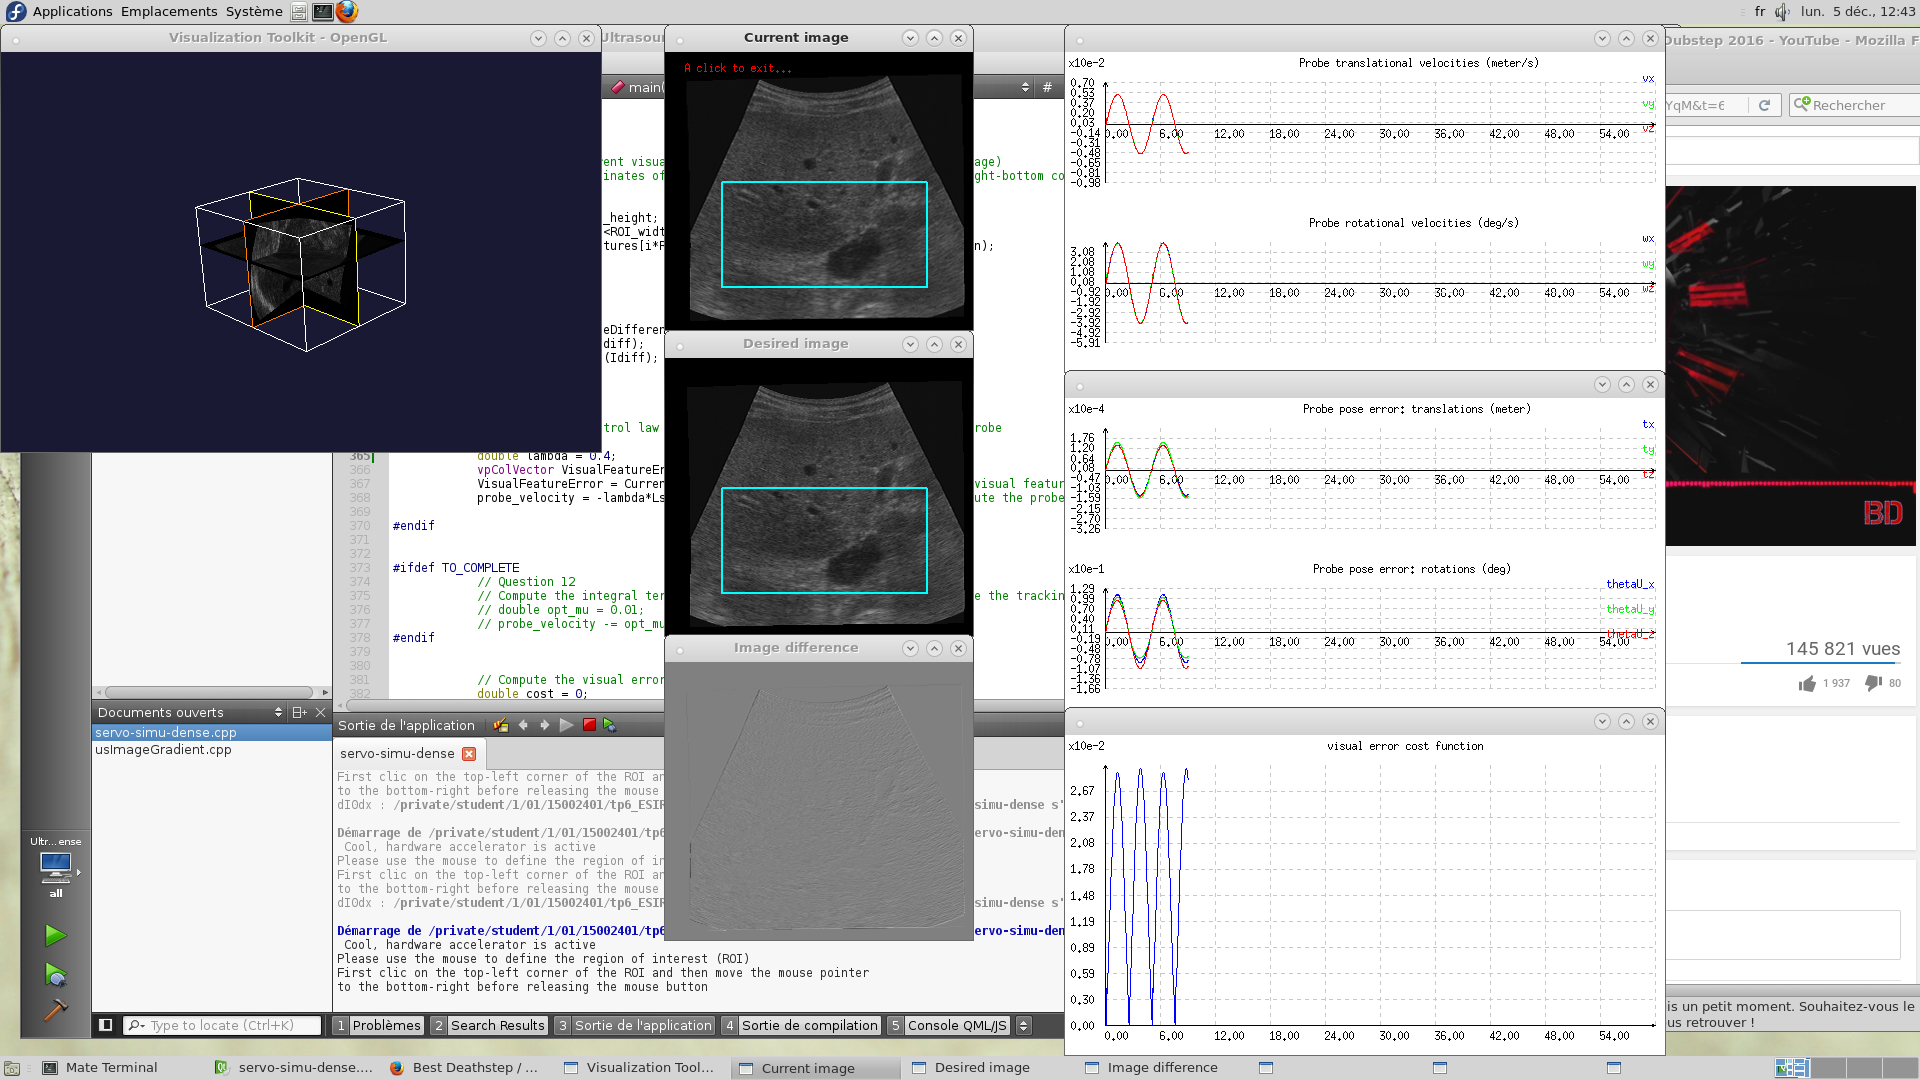
\includegraphics[width=1.0\textwidth]{./images/q8.png}
    \caption{Asservissement visuel}
    \label{assertVisu}
\end{figure}


\subsection{Question 9}
La region d'interet a beaucoup d'importance. Elle permet d'effectuer l'asservissement visuel correctement (ou non). Lorsque le ROI est grand, la loi de commande a peu de chance de se tromper de direction, parce le nombre de donn\'ees est tr\`es \'elev\'e. La minimisation de l'erreur fonctionne donc tr\`es bien (Figure \ref{largeRoi}). D\`es lors que le roi est r\'eduit, les pics de l'erreur sont plus \'elev\'es : 5.5x10-2 avec un ROI moyen contre 1.8x10-2 avec un grand ROI (figure \ref{mediumRoi}).
\par
Dans la m\^eme lign\'ee, l'erreur devient tr\`es forte lorsque le ROI est tr\`es petit (Figure \ref{smallRoi}). De plus, on constate m\^eme que dans ce cas l\`a, l'asservissement est imparfait : ça tremble. La r\'egion d'int\'er\^et \'etant tr\`es petite, les donn\'ees utiles pour l'asservissement sont pr\'esentes en petite quantit\'e, ce qui limite la pr\'ecision. Une r\'egion d'int\'er\^et de taille correcte est donc importante.

\begin{figure}[H]
    \centering
    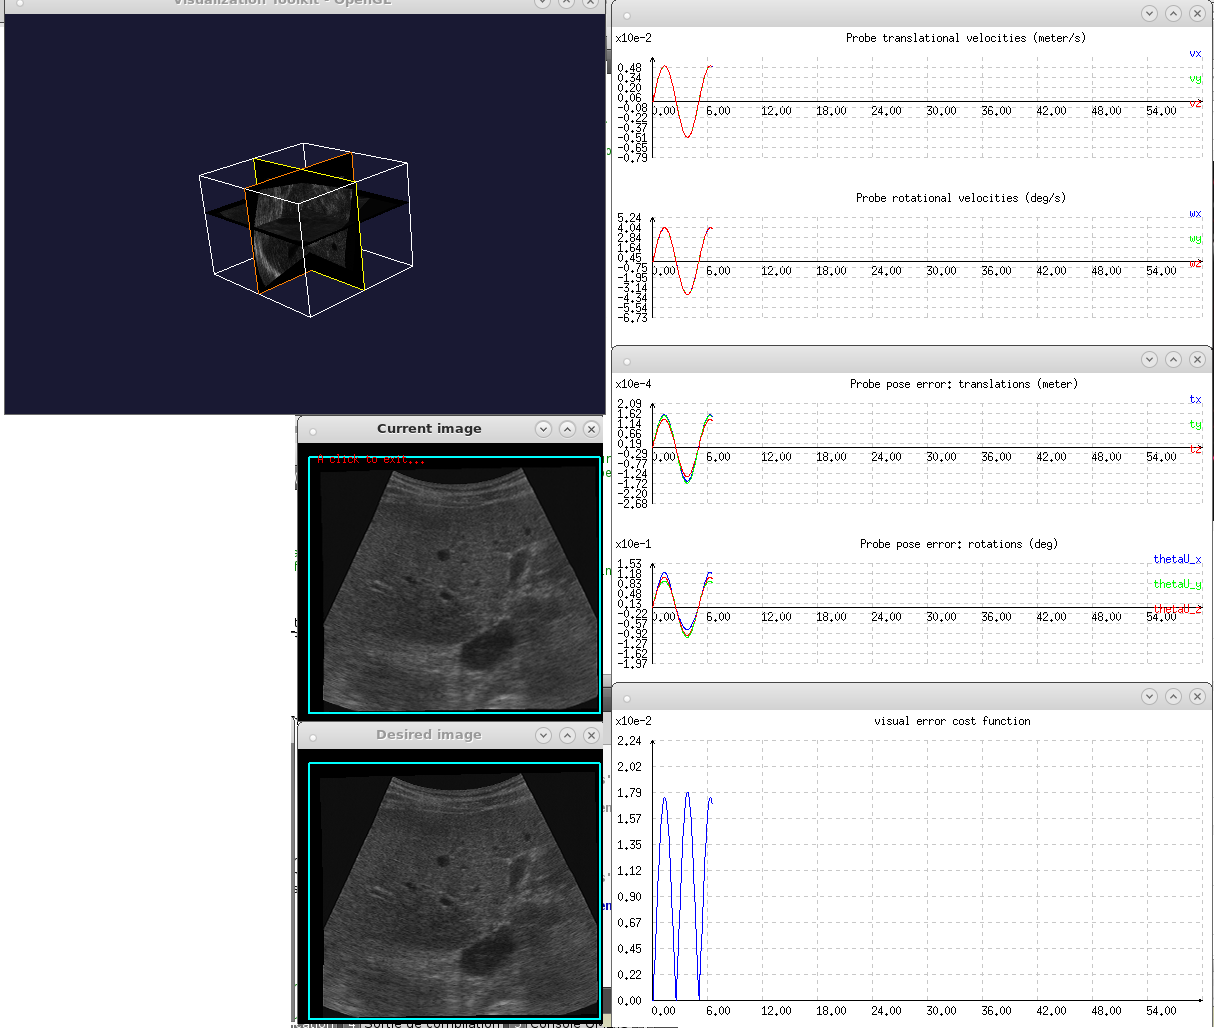
\includegraphics[width=0.5\textheight]{./images/q9_large.png}
    \caption{Asservissement avec un grand ROI}
    \label{largeRoi}
\end{figure}
\begin{figure}[H]
    \centering
    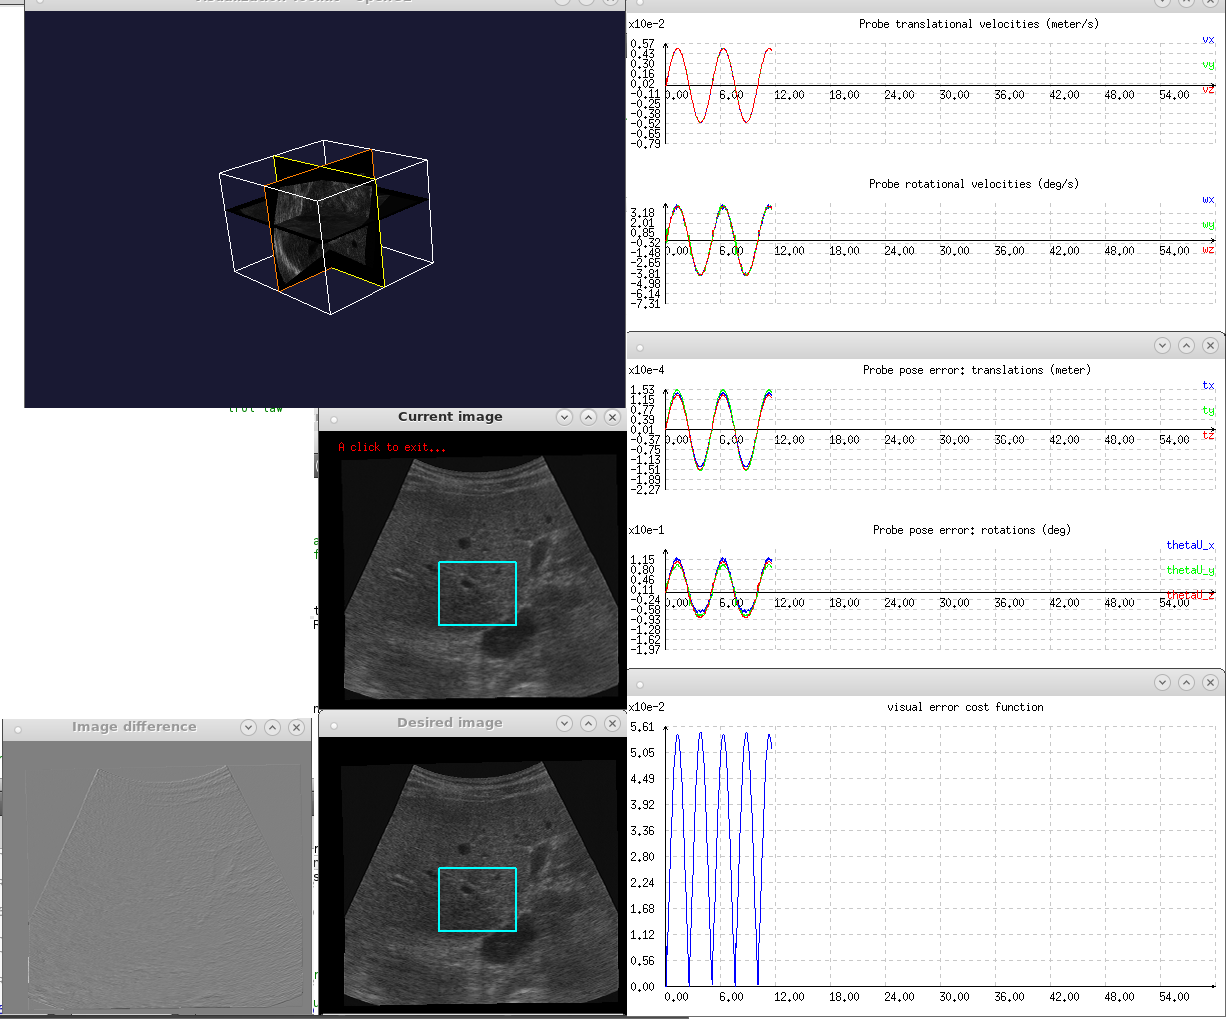
\includegraphics[width=0.5\textheight]{./images/q9_medium.png}
    \caption{Asservissement avec un ROI moyen}
    \label{mediumRoi}
\end{figure}
\begin{figure}[H]
    \centering
    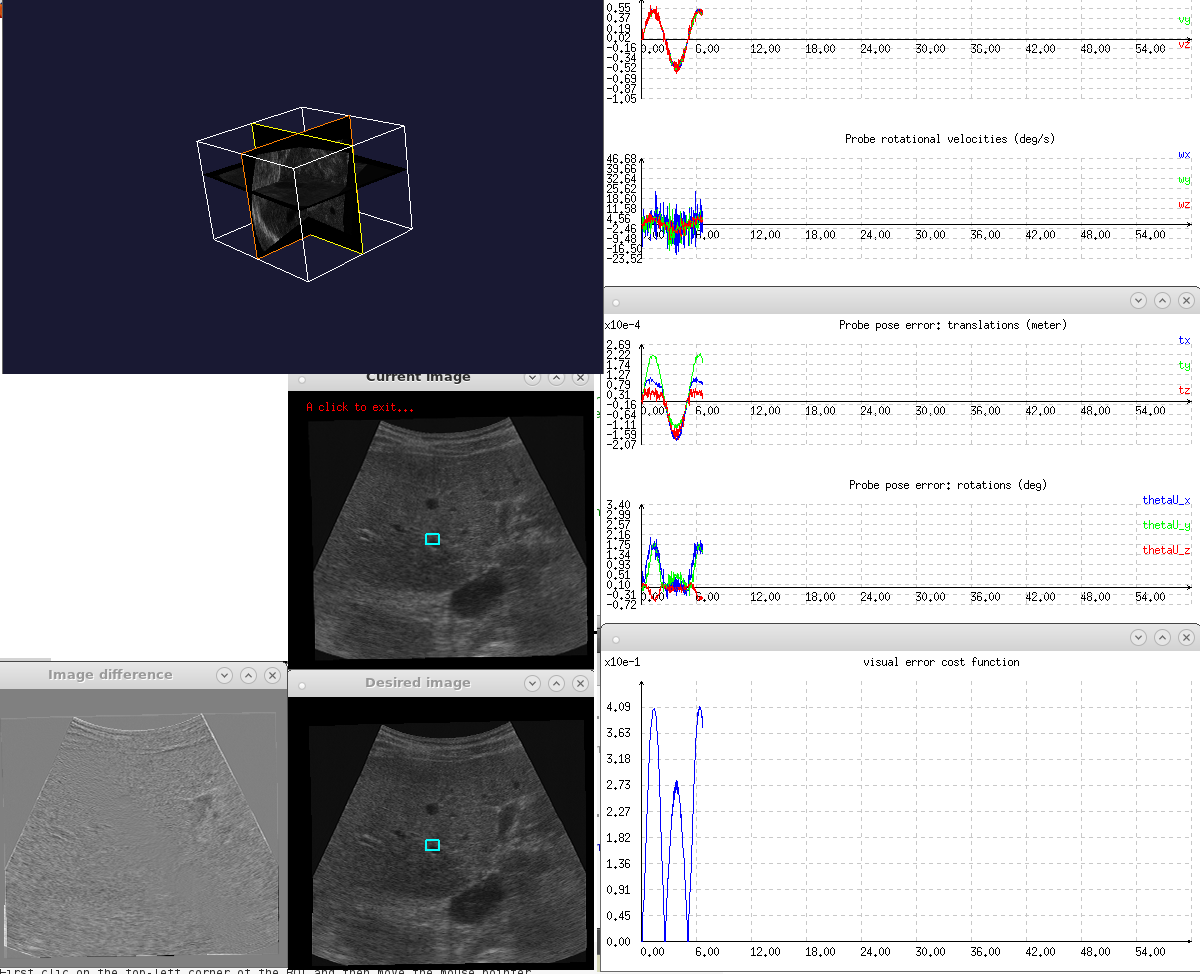
\includegraphics[width=0.5\textheight]{./images/q9_small.png}
    \caption{Asservissement avec un petit ROI}
    \label{smallRoi}
\end{figure}

\subsection{Question 10}
Lorsque le gain de contr\^ole est trop petit (lambda = 0.1), la cam\'era n'arrive \`a poursuivre l'objet en mouvement. Sa vitesse est trop faible par rapport au mouvement. L'erreur est donc \'elev\'ee en bout de l'oscillation, mais le re-postionnement est correct lorsque l'objet revient vers sa postion initiale (Figure \ref{smallGain}).
\par
A l'inverse, d\'efinir un gain de controle trop \'elev\'e entraine des vibrations : la cam\'era avance trop vite et se positionne incorrectement. R\'eguli\`erement, la cam\'era d\'epasse l'objet et est oblig\'ee de revenir sur ses pas. Cela provoque d'importants aller-retours visibles sur la figure \ref{bigGain}
\par
Le gain de contr\^ole maximum qui nous assure une compensation de mouvement correcte est lambda = 0.5.
\begin{figure}[H]
    \centering
    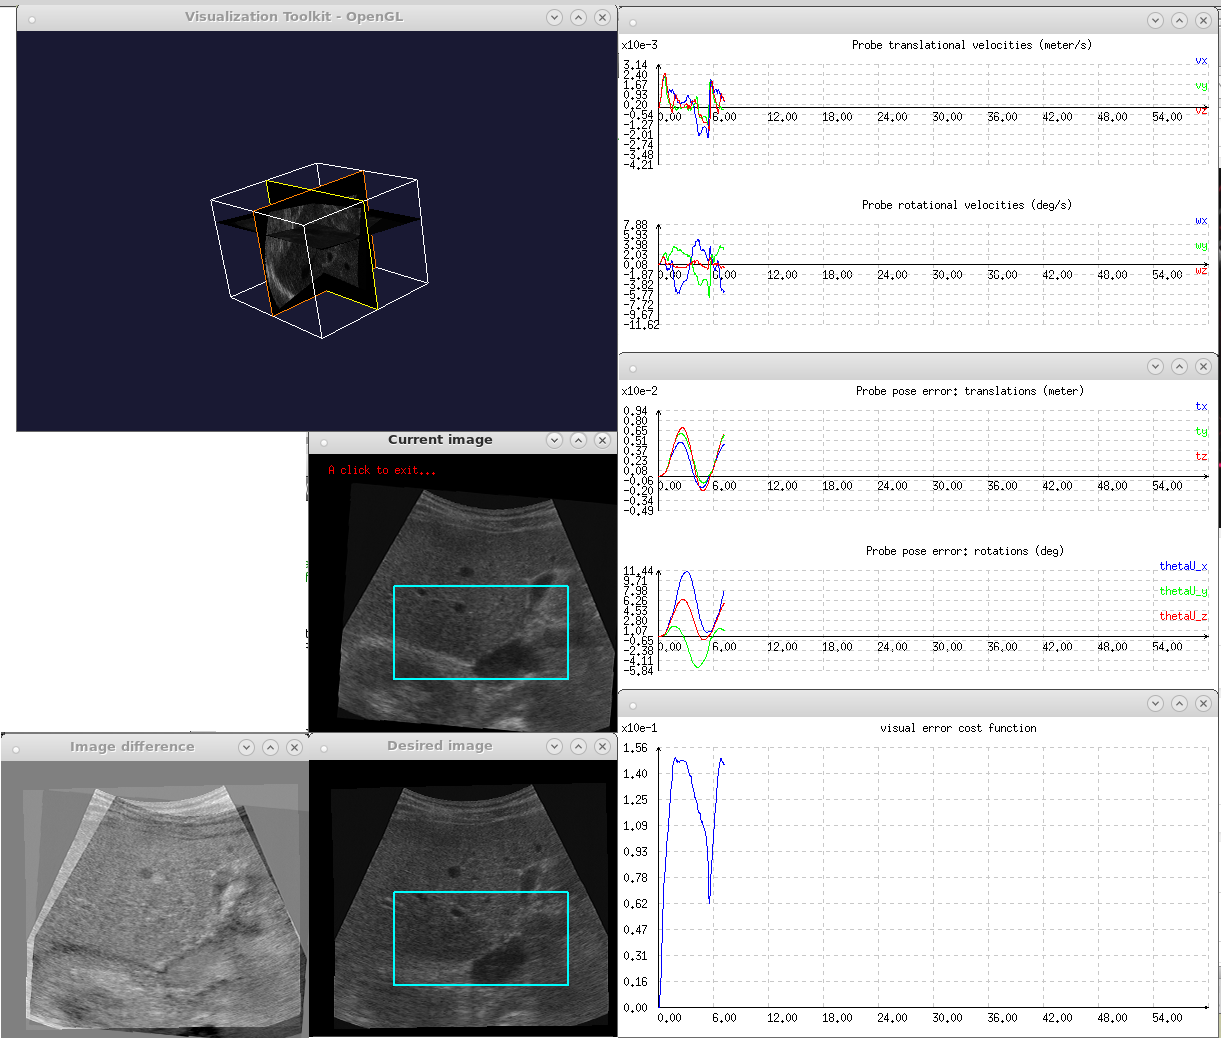
\includegraphics[width=0.5\textheight]{./images/q10_small.png}
    \caption{Asservissement avec un petit gain (lambda=0.1)}
    \label{smallGain}
\end{figure}
\begin{figure}[H]
    \centering
    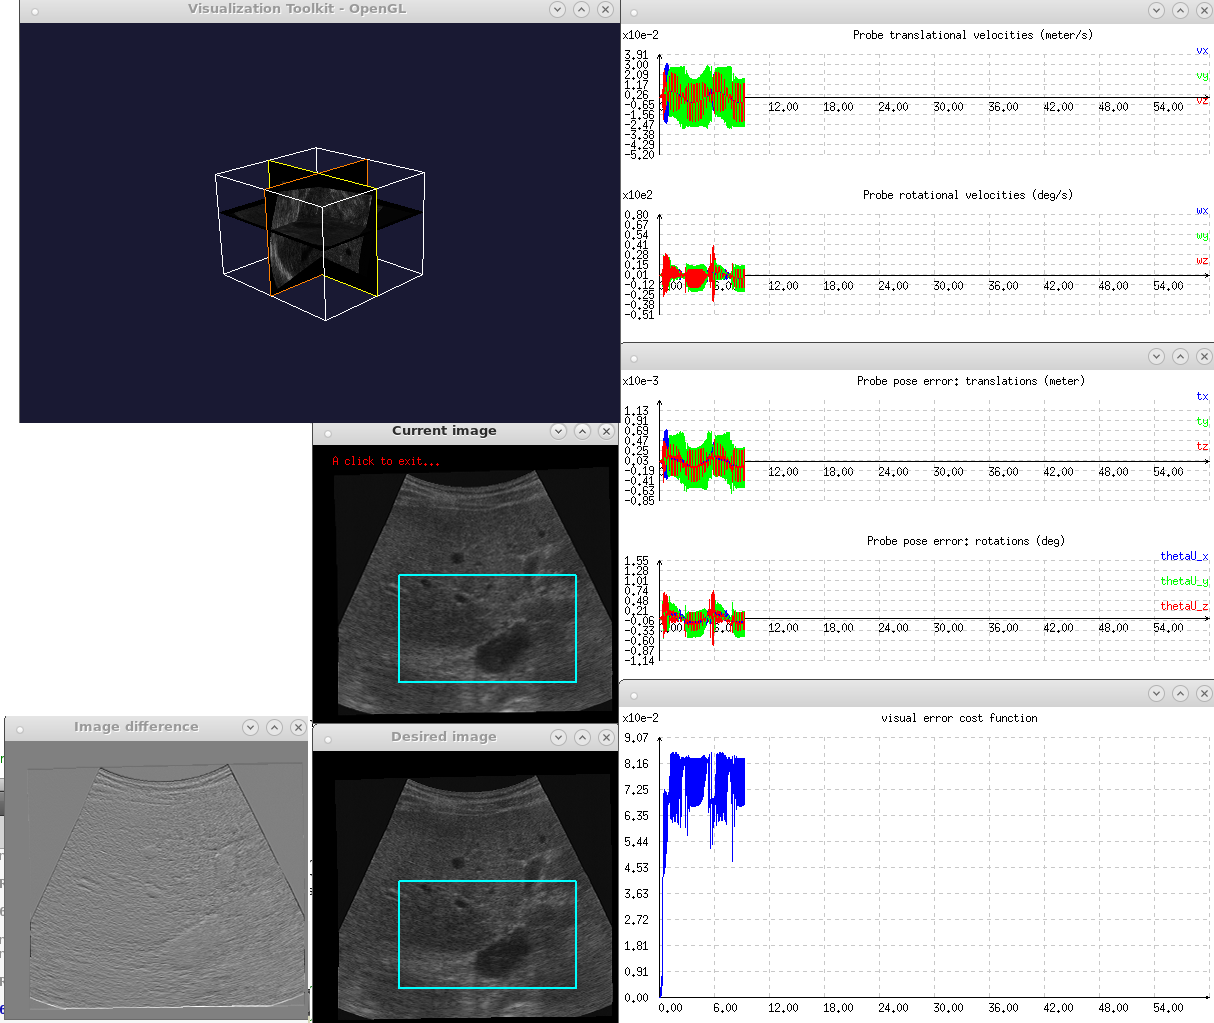
\includegraphics[width=0.5\textheight]{./images/q10_big.png}
    \caption{Asservissement avec un petit gain (lambda=0.8)}
    \label{bigGain}
\end{figure}

\subsection{Question 11}
Apr\`es l'acc\'el\'eration de l'amplitude du mouvement, on constate que l'asservissement visuel ne fonctionne plus. En effet, la vitesse (gain de contr\^ole) n'est plus du tout adapt\'ee au mouvement. Le plan de coupe se d\'esaxe rapidement et l'erreur explose. 
\par
Il est tr\`es difficle de trouver un gain de controle adapt\'e car, les oscillations ne sont pas de m\^eme taille selon les axes (de translation et de rotation). Un gain \'elev\'e entrainera une poursuite adapt\'ee sur un axe, mais trop trop rapide sur un autre.
\begin{figure}[H]
    \centering
    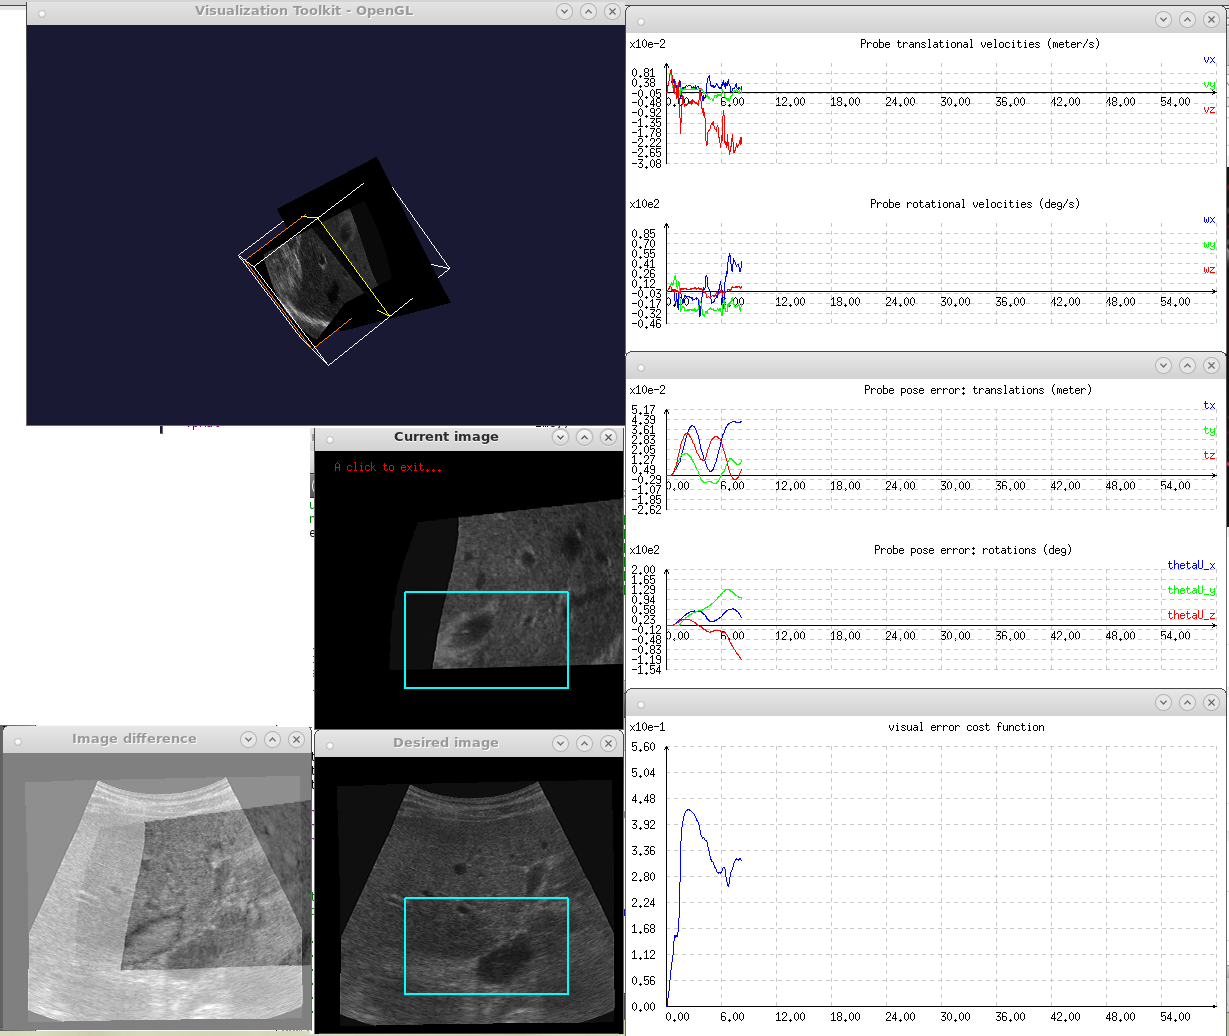
\includegraphics[width=0.5\textheight]{./images/q11_0,4.png}
    \caption{Asservissement avec mouvement rapide }
    \label{fastMove}
\end{figure}

\subsection{Question 12}
%TODO Expliquer le but de la question
\begin{verbatim}
%Mettre le code ici
\end{verbatim}
%TODO Commenter le code 

\subsection{Question 13}
%TODO

\section{Conclusion}
%TODO

\end{document}
\grid
\grid
